\section{Efficient Computations of Cryptographic Properties of S-Boxes} \label{sec:strength}
The strength of S-boxes can be measured in the context of Galois fields and Boolean functions. In this section, we focus on several important measurements of the cryptographic strength of S-boxes. We then present security metrics that can be used in the context of Boolean functions, such as nonlinearity, resiliency, the strict avalanche criterion, and algebraic immunity. We also present source code that may be used to efficiently compute such metrics.

\subsection{Linear Approximation and Difference Distribution}
With the advent of linear and differential cryptanalysis on SPN block ciphers, the contents of the linear approximation and difference distribution tables, which are highly dependent on the S-box used in such block ciphers, are critical in determining a particular construction's susceptibility to these attacks. Based on the definitions given in the preceding section, we can compute the $N_L(a,b)$ matrix using the procedure outlined in Algorithm \ref{alg:claAlg}. The exhaustive nature of this algorithm yields a time complexity of $\mathcal{O}(2^{4n})$. As such, when $n \approx 16$, computing this table cannot be done easily on a normal computer. An ideal S-box will have probabilities around 0.5 for all input and output combinations, meaning that linear combinations do not occur with non-random frequency, which is needed to carry out a successful linear cryptanalysis attack.

\begin{algorithm}[ht!] %[htb]
\caption{$N_L(S, n$)} \label{alg:claAlg}
\begin{algorithmic}[1]
\State $N_L \gets zeros(1...2^n - 1,1...2^n - 1)$
	\For {$a = 0 \text{ to } 2^n - 1$}
		\For {$b = 0 \text{ to } 2^n - 1$}
			\For {$x = 0 \text{ to } 2^n - 1$}
				\For {$y = 0 \text{ to } 2^n - 1$}
					\If {$S(x) = y$ and HW$((x \land a) \oplus (y \land b)) = 0$}
					% SumXOR(a,b,x,y) == 0$}
						\State $N_L(a,b) \gets N_L(a,b) + 1$
					\EndIf		
				\EndFor
			\EndFor
		\EndFor
	\EndFor
% \\
% 	\Function{SumXOR}{$a,b,x,y$}
% 		\State $x' = x \land a$ \Comment {$a \cdot x$}
% 		\State $y' = y \land b$ \Comment {$b \cdot y$}
% 		\State \Return HW$(x' \oplus y')$ 
% 	\EndFunction
\end{algorithmic}
\end{algorithm}

As discussed in the previous section, differential cryptanalysis relies on the difference distribution table, $N_D(\Delta X, \Delta Y)$. Since this table is generated from an exhaustive check of all input and output differences, we compute it very similar to $N_L(a,b)$ using Algorithm \ref{alg:ddtable}. However, we now only have a time complexity of $\mathcal{O}(2^{2n})$.

\begin{algorithm}[ht!]
\caption{$N_D(S, n)$} \label{alg:ddtable}
\begin{algorithmic}[1]
\State $N_D \gets zeros(1...2^n - 1,1...2^n - 1)$
\For {$x_1 = 0 \text{ to } 2^n - 1$}
	\For {$x_2 = 0 \text{ to } 2^n - 1$}
		\State $\Delta X = x_1 \oplus x_2$
		\State $\Delta Y = S(x_1) \oplus S(x_2)$
		\State $N_D[\Delta X, \Delta Y] \gets N_D[\Delta X, \Delta Y] + 1$
	\EndFor
\EndFor
\State \Return $N_D$
\end{algorithmic}
\end{algorithm}

\subsection{Nonlinearity}
Since Boolean functions are natural representations for S-boxes, the nonlinearity of Boolean functions becomes fundamental in the assessment of the cryptographic strength of S-boxes. This is particularly true with the advent of linear cryptanalysis attacks. Intuitively, a higher measure of nonlinearity means that linear approximations of an $n$-bit S-box will be satisfied with less frequency, which means that there will be less input and output sums for the S-box with high magnitude biases. This will typically lead to more evenly distributed entries in the $N_L(a,b)$ table that are close to $2^{n-1}$, which yield biases of $0$.

For a Boolean function $f$, the nonlinearity $\mathcal{N}_l$ is defined as the minimum distance between $f$ and all possible affine functions on $n$ variables. Formally, we define the nonlinearity as follows \cite{cusik09-BooleanFunctions}:
\begin{align*}
\mathcal{N}_l(f) = \min_{\phi \in \Omega_n} d(f, \phi),
\end{align*}
where $d(f, g) = $HW$(f \oplus g)$ (i.e. the Hamming distance between two functions $f$ and $g$). The maximum value for $\mathcal{N}_l$ is $2^{n-1} - 2^{n/2 - 1}$.
It is also convenient to use the Walsh-Hadamard transform of a Boolean function $f$ as $W_f(u) = \sum_{x \in \mathbb{F}_2^n} (-1)^{f(x) \oplus (u \cdot x)}$, where $w \in \mathbb{F}_2^n$ and $w \cdot x$ is the inner product of the two vectors $w, x \in \mathbb{F}_2$ \cite{cusik09-BooleanFunctions}, to define the nonlinearity of a function $f$ as 
\begin{equation} \label{eqn:nlFromWalsh}
\mathcal{N}_l(f) = 2^{n-1} - \frac{1}{2}\max_{u \in \mathbb{F}_2^n}|W_f(u)|.
\end{equation}
If $n$ is odd then a Boolean function $f$ is called maximally nonlinear if every element of the Walsh spectrum belongs to the set $\{0, \pm 2^{(n+1)/2}\}$ \cite{Nawaz09-1}. The same cannot be said for even values of $n$, which are of interest in this work. It has been conjectured that a maximum upper bound on the nonlinearity for such functions is $2^{n-1} - 2^{n/2}$, and we call a function $F$ \emph{maximally nonlinear} if it reaches this bound \cite{Dobbertin99-1}. Maximally nonlinear Boolean functions are also called \emph{bent functions}, and were first introduced by Rothaus in 1976 \cite{Rothaus76-1}. Nyberg studied the properties and constructions of bent functions using the discrete Fourier transform in \cite{Nyberg91-1}. Inspired by the notion of perfect nonlinearity, we measured the nonlinearity of all bijective S-boxes over $GF(2^8)$. The results of this experiment are shown in Chapter \ref{chp:results}.

In order to efficiently compute the nonlinearity of a Boolean function we use the Fast Walsh Transform (FWT) to compute the Walsh spectrum of Boolean function \cite{Shanks69-1}. A visual depiction of how this algorithm operates given the truth table representation for a Boolean function is shown in Figure \ref{fig:fwt}. It is well known that the time complexity of the FWT is $\mathcal{O}(n \ln n)$ (as observed in the visual example). To illustrate this complexity, our Python code that implements the FWT is shown in Listing \ref{lst:fwt}.

\begin{figure}
\centering
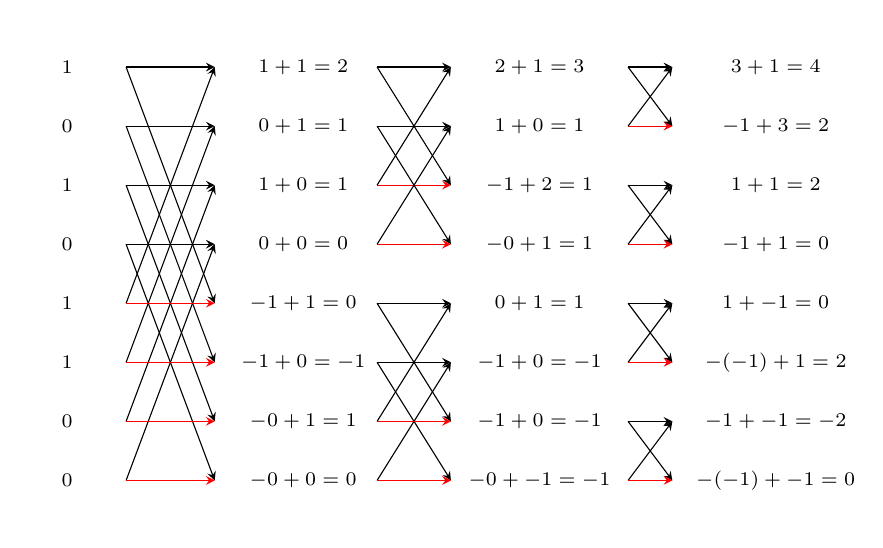
\begin{tikzpicture}
[bend angle =60,inner sep=0pt, minimum size =10mm,very thick,
from/.style={<-},
towards/.style={->},
field/.style={},
sub/.style={draw, thin, color=red, ->, >=stealth},
add/.style={draw, thin, color=black,->, >=stealth},
scale=0.75]
\node[field] (f18) at (0,8) {\scriptsize 1};
\node[field] (f17) at (0,7) {\scriptsize 0};
\node[field] (f16) at (0,6) {\scriptsize 1};
\node[field] (f15) at (0,5) {\scriptsize 0};
\node[field] (f14) at (0,4) {\scriptsize 1};
\node[field] (f13) at (0,3) {\scriptsize 1};
\node[field] (f12) at (0,2) {\scriptsize 0};
\node[field] (f11) at (0,1) {\scriptsize 0};

\node[field] (f28) at (4,8) {\scriptsize $1+1 = 2$};
\node[field] (f27) at (4,7) {\scriptsize $0+1=1$};
\node[field] (f26) at (4,6) {\scriptsize $1+0=1$};
\node[field] (f25) at (4,5) {\scriptsize $0+0=0$};
\node[field] (f24) at (4,4) {\scriptsize $-1+1=0$};
\node[field] (f23) at (4,3) {\scriptsize $-1+0=-1$};
\node[field] (f22) at (4,2) {\scriptsize $-0+1=1$};
\node[field] (f21) at (4,1) {\scriptsize $-0+0=0$};

\node[field] (f38) at (8,8) {\scriptsize $2+1=3$};
\node[field] (f37) at (8,7) {\scriptsize $1+0=1$};
\node[field] (f36) at (8,6) {\scriptsize $-1+2=1$};
\node[field] (f35) at (8,5) {\scriptsize $-0+1=1$};
\node[field] (f34) at (8,4) {\scriptsize $0+1=1$};
\node[field] (f33) at (8,3) {\scriptsize $-1+0=-1$};
\node[field] (f32) at (8,2) {\scriptsize $-1+0=-1$};
\node[field] (f31) at (8,1) {\scriptsize $-0+-1=-1$};

\node[field] (f48) at (12,8) {\scriptsize $3+1=4$};
\node[field] (f47) at (12,7) {\scriptsize $-1+3=2$};
\node[field] (f46) at (12,6) {\scriptsize $1+1=2$};
\node[field] (f45) at (12,5) {\scriptsize $-1+1=0$};
\node[field] (f44) at (12,4) {\scriptsize $1+-1=0$};
\node[field] (f43) at (12,3) {\scriptsize $-(-1) + 1 = 2$};
\node[field] (f42) at (12,2) {\scriptsize $-1 + -1 = -2$};
\node[field] (f41) at (12,1) {\scriptsize $-(-1) + -1 = 0$};

% PASS 1
\draw [add] (1,8) -- (2.5,8);
\draw [add] (1,7) -- (2.5,7);
\draw [add] (1,6) -- (2.5,6);
\draw [add] (1,5) -- (2.5,5);

\draw [add] (1,8) -- (2.5,4);
\draw [add] (1,7) -- (2.5,3);
\draw [add] (1,6) -- (2.5,2);
\draw [add] (1,5) -- (2.5,1);

\draw [add] (1,4) -- (2.5,8);
\draw [add] (1,3) -- (2.5,7);
\draw [add] (1,2) -- (2.5,6);
\draw [add] (1,1) -- (2.5,5);

\draw [sub] (1,4) -- (2.5,4);
\draw [sub] (1,3) -- (2.5,3);
\draw [sub] (1,2) -- (2.5,2);
\draw [sub] (1,1) -- (2.5,1);

% PASS 2
\draw [add] (5.25,8) -- (6.5,8);
\draw [add] (5.25,7) -- (6.5,7);
\draw [sub] (5.25,6) -- (6.5,6);
\draw [sub] (5.25,5) -- (6.5,5);

\draw [add] (5.25,8) -- (6.5,6);
\draw [add] (5.25,7) -- (6.5,5);
\draw [add] (5.25,6) -- (6.5,8);
\draw [add] (5.25,5) -- (6.5,7);

\draw [add] (5.25,4) -- (6.5,2);
\draw [add] (5.25,3) -- (6.5,1);
\draw [add] (5.25,2) -- (6.5,4);
\draw [add] (5.25,1) -- (6.5,3);

\draw [add] (5.25,4) -- (6.5,4);
\draw [add] (5.25,3) -- (6.5,3);
\draw [sub] (5.25,2) -- (6.5,2);
\draw [sub] (5.25,1) -- (6.5,1);

% PASS 3
\draw [add] (9.5,8) -- (10.25,8);
\draw [sub] (9.5,7) -- (10.25,7);
\draw [add] (9.5,6) -- (10.25,6);
\draw [sub] (9.5,5) -- (10.25,5);

\draw [add] (9.5,8) -- (10.25,7);
\draw [add] (9.5,7) -- (10.25,8);
\draw [add] (9.5,6) -- (10.25,5);
\draw [add] (9.5,5) -- (10.25,6);

\draw [add] (9.5,4) -- (10.25,3);
\draw [add] (9.5,3) -- (10.25,4);
\draw [add] (9.5,2) -- (10.25,1);
\draw [add] (9.5,1) -- (10.25,2);

\draw [add] (9.5,4) -- (10.25,4);
\draw [sub] (9.5,3) -- (10.25,3);
\draw [add] (9.5,2) -- (10.25,2);
\draw [sub] (9.5,1) -- (10.25,1);

% \draw[->] (e1) -- +(0pt,-25pt);
% \draw[->] (e2) -- +(0pt,25pt);
\end{tikzpicture}
\label{fig:fwt}
\caption{Visual depiction of the Fast Walsh Transform that is used to calculate the Walsh spectrum for the Boolean function $f = (10101100)$.}
\end{figure}

% \begin{code}
% \begin{minted}[frame=single]{py}
% def my_func(x):
%     print x
% \end{minted}
% \caption{My Func}
% \label{lst:my_func}
% \end{code}

% \begin{listing}[frame=single]
% \begin{code}
\begin{listing}[ht!]
\caption{Python source code to compute the FWT for a Boolean function $f$.}
\begin{minted}[fontsize=\scriptsize]{python}
def fwt(f): # f is a Boolean function represented as a TT of length 2^n
	wf = []
	for x in f:
		if x == 0:
			wf.append(1)
		else: # Assume a proper truth table of only 1 or 0 entries
			wf.append(-1)
	k = len(f) # k = 2^n
	n = int(math.log(k, 2))
	sw = 1
	bs = k - 1
	while True:
		li = 0
		bs = bs >> 1
		for b in range(bs, -1, -1):
			ri = li + sw
			for p in range(0, sw):
				a = wf[li]
				b = wf[ri]
				wf[li] = a + b
				wf[ri] = a - b
				li = li + 1
				ri = ri + 1
			li = ri
		sw = (sw << 1) & (k - 1)
		if (sw == 0):
			break
	return wf
\end{minted}
\label{lst:fwt}
\end{listing} 
% \end{code}
% \label{lst:fwt}
% \end{listing} 

Given the definition of nonlinearity based on the Walsh transform in Equation \ref{eqn:nlFromWalsh}, we may compute the nonlinearity of a Boolean function by taking the FWT of its truth table and then subtracting half of the maximum absolute value entry in the output vector from $2^{n-1}$. We may use this same approach to compute the nonlinearity of an S-box. First, observe that the definition of nonlinearity for one-dimensional Boolean functions naturally extends to the nonlinearity of $(n,m)$-Boolean functions, denoted as $\mathcal{N}_l(F)$, by considering the minimum nonlinearity over all linear combinations of the $m$ coordinate functions of $F$. We formalize this definition in the following \cite{Carlet10-1}: 
\begin{align*}
\mathcal{N}_l(F) = \min_{c \in \mathbb{F}_2^m}\{\mathcal{N}_l(c \cdot F)\} = \min_{c \in \mathbb{F}_2^m}\{\mathcal{N}_l(c_0f_0 \oplus c_1f_1 \oplus \dotsb \oplus c_{m-1}f_{m-1})\}
\end{align*}
Cryptographically strong S-boxes have high measures of nonlinearity, meaning that it is increasingly difficult to approximate the S-box using a linear affine function. When constructing S-boxes we must consider this as one of the primary metrics to optimize. To do so, we used the snippet of Python code in Listing \ref{lst:nonlinearityCode} to compute the nonlinearity of an $(n,n)$ S-box, which essentially finds the minimum nonlinearity among all $2^n - 1$ non-zero linear combinations of the coordinate functions of the S-box using the FWT.

\begin{listing}[ht!]
\caption{Python source code to compute the nonlinearity of an $(n, n)$ S-box.}
\begin{minted}[fontsize=\scriptsize]{python}
def bf_nonlinearity(f, n):
	fw = fwt(f)
	for i in range(len(fw)):
		fw[i] = abs(fw[i])
	return ((2**(n-1)) - (max(fw) / 2)) # nonlinearity from the Walsh transform
def nonlinearity(S):
	order = len(S)
	n = int(math.log(order, 2))
	nl = 1 << order # over the top
	for mask in range(1, order): 
		f = []
		for x in range(0, order): 
			s = 0
			for i in range(0, n):
				if ((mask & (1 << i)) > 0) and ((S[x] & (1 << i)) > 0):
					s = s ^ 1;
			f.append(s)
		bfnl = bf_nonlinearity(f, n)
		if (bfnl < nl):
			nl = bfnl 
	return nl
\end{minted}
\label{lst:nonlinearityCode}
\end{listing}
% \end{lstlisting} \label{lst:nonlinearity}

% More specifically, differential cryptanalysis relies on an uneven distribution in the cardinality of the set $\{D_{\alpha}S(x) : x,\alpha \in GF(2^n)\}$.
%TODOTODO: replace all F's by S

\subsection{Differential Uniformity}
First introduced in 1994 by Nyberg \cite{Nyberg94-1}, we say that an S-box $S : GF(2^n) \to GF(2^m)$ is $\delta$-differentially uniform if for all $\alpha \in GF(2^n)$ and $\beta \in GF(2^m)$ we have
\begin{align*}
|\{x \in GF(2^n) | D_{\alpha}S(x) = \beta\}| \leq \delta, 
\end{align*}
where $D_{\alpha}S(x) = S(x + \alpha) + S(x)$, $\alpha \in GF(2^n)$, and $\beta \in GF(2^m)$. Equivalently, we say that such an S-box $S : GF(2^n) \to GF(2^m)$ is $\delta$-differentially uniform if $S(x + \alpha) + S(x) = \beta$ has at most $\delta$ solutions in $GF(2^n)$. Differential cryptanalysis exploits the lack of uniformity in the nonlinear S-box step of SPN block ciphers. Intuitively, an uneven distribution implies that there exists a single element $\beta \in GF(2^m)$ that is mapped to with higher frequency given two different input elements $x$ and $\alpha$. In an ideal SPN block cipher, the probability that a given input difference $\Delta X$ will yield a specific output difference $\Delta Y$ should be exactly $2^{-n}$, where $n = m$ is the size of the input and output elements. If an S-box is not differentially 1-uniform, then there will exist a value $\beta \in GF(2^m)$ such that for any two randomly selected input elements $x$ and $\alpha$, $ D_{\alpha}S(x) = \beta$ will be the output more than once. From an attacker's perspective, this means that there will exist an output difference $\Delta Y$ that occurs with higher probability for a select of input differences $\Delta X$.

Cryptographically strong S-boxes have low values for $\delta$, as this means the output of $S$ is relatively uniform and the frequency of a single output value cannot be easily exploited for an attack. Differential uniformity was first studied in the context of the Data Encryption Standard, and it was proven in \cite{Nyberg94-1} that if the round functions of Feistel-based ciphers similar to DES are $\delta$-differentially uniform, then the average probability to obtain a non-zero output for input $x + \alpha$, for all $x, \alpha \in GF(2^n)$, after 4 rounds (in a DES-like cipher) is bounded by $2(\frac{\delta}{2^n})^2$.

Functions achieving this bound with $\delta = 1$ are referred to as \emph{perfectly nonlinear}. Functions achieving this bound with $\delta = 2$ are referred to as \emph{almost perfectly nonlinear} functions \cite{Nyberg91-1}. In practice, S-boxes with $\delta \in \{1,2\}$ are rarely used because functions with simple algebraic expressions that exhibit this property are difficult to find. Instead, S-boxes with $\delta=4$ are quite common due to the use of the inverse power mapping in the AES \cite{Daemen02-1}. More specifically, S-boxes of the form $S(x) : x^{-1}$ were shown to have $\delta = 4$ with a $\mathcal{N}_l$ lower bound of $2^{n-1} - 2^{\frac{n}{2}}$ in \cite{Nyberg94-1}. 

% Similarly, S-boxes of the form $S(x) = x^{2^{k} + 1}$ have $\delta = 2$ with $\mathcal{N}_l$ equal to precisely $2^{n-1} - 2^{\frac{n-1}{2}}$. As a result, these are classified as cryptographically strong power mappings, which is a topic we will revisit in Chapter \ref{chp:sboxConstruction}.

Our Python code to compute the differential uniformity of an S-box $S : GF(2^n) \to GF(2^n)$ is shown in Listing \ref{lst:duCode}. Given the exhaustive nature of this algorithm, its time complexity is on the order of $\mathcal{O}((2^n)^3) = \mathcal{O}(2^{3n})$, making it a computationally difficult procedure for large values of $n$. The time complexity is quite reasonable for $n = 8$, and as a result, we used this procedure to compute $\delta$ for all bijective power mappings over $GF(2^8)$. The results of this experiment are discussed in Chapter \ref{chp:results}.

% \begin{lstlisting}[
%\ref{lst:differentialUniformity}
\begin{listing}[ht!]
\caption{Python code to compute the differential uniformity $\delta$ of an $(n, n)$ S-box.}
\begin{minted}[fontsize=\scriptsize]{python}
def differentialUniformity(S):
	c = 0
	delta = 0
	n = len(S)
	for alpha in range(1, n): 
		for beta in range(n):
			c = 0
			for z in range(n):
				if ((S[(z ^ alpha)] ^ S[z]) == beta):
					c = c + 1
			if (c > delta): 
				delta = c
	return delta 
\end{minted}
\label{lst:duCode}
\end{listing}
% \end{lstlisting} \label{lst:differentialUniformity}

\subsection{Resiliency}
Resiliency is a combination of balancedness and correlation immunity. Balancedness is a simple property of Boolean functions; a Boolean function is balanced if the (Hamming) weight of its truth table vector is $2^{n - 1}$. A Boolean function $f$ on $n$ variables is said to have a correlation immunity of order $t$, $1 \leq t \leq n$, if the output is statistically independent for any fixed subset of at most $t$ variables. In other words, the output distribution probability is unchanged when at most $t$ input variables are kept constant. A Boolean function is said to be $t$-resilient if it is $t$-correlation immune (CI) and balanced. Similar to the nonlinearity metric for $(n,m)$ Boolean functions, an $(n,m)$ Boolean function $F$ is said to be $t$ correlation immune if and only if all $2^m - 1$ Boolean functions $v \cdot F, v \in \mathbb{F}_2^{m*}$ are $t$-th order correlation immune, and similarly, $F$ is $t$-resilient if and only if all functions $2^m - 1$ Boolean functions $v \cdot F, v \in \mathbb{F}_2^{m*}$ are $t$-resilient \cite{Carlet04-1}. Resiliency is an important property of cryptosystems with the advent of correlation attacks on stream ciphers \cite{Canteaut05-1} (a topic we omitted from the previous section), which can be deterministically transformed to block ciphers and vice versa. Higher orders of resiliency, and as a result, correlation immunity, are ideal for S-boxes.

Fortunately, there exists a very efficient way to determine if a Boolean function $f$ is $t$-CI using its Walsh spectrum \cite{Gao11-1}. In particular, it is a known fact that $f$ is $t$-CI if and only if $W_f(u) = 0$ for all $u \in \mathbb{F}_2^n$, $1 \leq $HW$(u) \leq t$. Furthermore, by the properties of the Walsh transform, $f$ is balanced if and only if $W_f(\bar{0}) = 0$. Using these two facts, we may easily determine the maximum $t$ such that $f$ is $t$-CI and $t$-resilient using the two snippets of code shown in Listings \ref{lst:CIcode} and \ref{lst:resiliencyCode}. 

\begin{listing}[ht!]
\caption{Python code to compute the correlation immunity of an $(n, n)$ S-box.}
\begin{minted}[fontsize=\scriptsize]{python}
def correlationImmunity(S):
	order = len(S)
	n = int(log(order, 2))
	for t in range(n):
		if isCorrelationImmune(S, order, n, t) == False:
			return t - 1
def isCorrelationImmune(S, order, n, t):
	for mask in range(1, order): # omit the 0 function
		f = []
		for x in range(0, order):
			s = 0
			for i in range(0, n):
				if ((mask & (1 << i)) > 0) and ((S[x] & (1 << i)) > 0):
					s = s ^ 1
			f.append(s)
		spectrum = fwt(f)
		for x in range(order):
			if (wt(x) <= t and spectrum[x] != 0):
				return False
	return True
\end{minted}
\label{lst:CIcode}
\end{listing}

% \begin{lstlisting}[
\begin{listing}[ht!]
\caption{Python code to compute the resiliency of an $(n, n)$ S-box.}
\begin{minted}[fontsize=\scriptsize]{python}
def resiliency(S):
	order = len(S)
	n = int(math.log(order, 2))
	for t in range(n):
		for mask in range(1, order): # omit the 0 function
			f = []
			for x in range(0, order):
				s = 0
				for i in range(0, n):
					if ((mask & (1 << i)) > 0) and ((S[x] & (1 << i)) > 0):
						s = s ^ 1
				f.append(s)
			spectrum = fwt(f)
			if (spectrum[0] == 0): # balanced
				for u in range(order):
					if (wt(u) <= t and spectrum[u] != 0):
						return t - 1
			else:
				return t - 1
\end{minted}
\label{lst:resiliencyCode}
\end{listing}
% \end{lstlisting} \label{lst:resiliency}

With a time complexity of $\mathcal{O}(n \ln n)$ for the FWT, it is easy to see that each of these procedures has a time complexity of $\mathcal{O}(n(2^{n}(2^n(n\ln n)2^n))) = \mathcal{O}(n^2\ln n 2^{3n})$. The exponential complexity comes from the fact that for every $2^n$ linear combinations of the $n$ coordinate functions of the $S$ we must compute a new Boolean function of size $2^n$, perform the FWT, and then check all $2^n$ entries of the Boolean function to see if those indexes with weight at most $t$ have a non-zero value in the Walsh spectrum. We did not explore further optimizations to these procedures. 

\subsection{Algebraic Immunity}
This metric is used to determine a Boolean functions resilience to attacks based on annihilators, which are used to deduce a multivariate equation in the output of the function that have a low enough degree to solve efficiently. Formally, an annihilator of a Boolean function $f$ is another a Boolean function $g$ such that $f \oplus g = 0$. Using low-degree annihilators it is sometimes possible to reduce the degree of a Boolean function in a system of multivariate equations to a small enough value such that the system of equations relating the Boolean function and state bits of a cryptosystem can be solved in a reasonable amount of time. Motivated by the presence of low-degree annihilators, the component algebraic immunity $AI_c(S)$ of an $(n,m)$ S-box $F$ is then defined in terms of the algebraic immunity $AI$ of the $m$ component functions as follows: 
\begin{align*}
AI_c = \min_{c \in \mathbb{F}_2^m}\{AI(c \cdot F)\} = \min_{c \in \mathbb{F}_2^m}\{AI(c_0f_0 \oplus c_1f_1 \oplus \dotsb \oplus c_{m-1}f_{m-1})\} 
\end{align*}
It is important to note that this metric is only really suited for LFSR-based ciphers, which is why we did not discuss this type of algebraic attack in the preceding section. The concept of algebraic immunity for block ciphers not constructed on LFSRs has since been modified due to the introduction of the XL and XSL attacks by Courtois et al. \cite{Courtois02-1}. As the XL and XSL are algebraic attacks, their establishment led to a new notion of algebraic immunity, which Courtois et al. defined as the values $\Gamma(r, s, t) = (t/s)^{\lceil t/r \rceil}$ and $\Gamma'(r,s,t) = ((t - r)/s)^{\lceil (t - r)/s \rceil}$. These metrics denote the resistance of an S-box (used in block ciphers) against the XSL attacks, where $r$ is the number equations that represent the S-box, $s$ is the size (in bits) of the S-box (i.e. $s = n$), and $t$ is the number of terms - the sparsity of terms - that appear in the $r$ equations. The difference between $\Gamma$ and $\Gamma'$ depends on the type of XSL attack; $\Gamma$ corresponds to the attack that exploits knowledge of the key schedule of a block cipher, whereas $\Gamma'$ does not rely on such information and, as a result, is more of theoretical interest. If biaffine equations are used in the XSL attack, then $t = s(s + 2) + 1$, and if fully quadratic equations are used in the XSL attack, then $t = s(2s + 1) + 1$ \cite{Courtois05-1}. If we know the dimension of the S-box $s$, then the only remaining task is to determine $r$, the number of linearly independent biaffine or fully quadratic equations. Courtois proved exact values for $r$ for a variety of cryptographically significant power mappings in \cite{Courtois05-1}. Building upon this work, Yassir \cite{Nawaz09-1} generalized these results into an algorithm to compute the number of linearly biaffine and fully quadratic equations for arbitrary power mappings, which are transcribed in Algorithms \ref{alg:biaffineNumber} and \ref{alg:quadraticNumber}, respectively. Both of these algorithms have a very efficient time complexity of $\mathcal{O}(n^2)$, making it very easy to determine the effectiveness of the XSL attack on a particular S-box used in a block cipher. 

\begin{algorithm}[ht!] %[htb]
\caption{Number of Linearly Independent Bi-Affine Equations (modified from \cite{Nawaz09-1})} 
\label{alg:biaffineNumber}
\begin{algorithmic}[1]
	\Require{$a$, $n > 1$}
	\State $cst_l \gets []$
	\State $cst_s \gets []$
	\State $cs \gets Coset(a, 2^n - 1)$ %, cst_l \gets Append(cst_l, Min(cs)),cst_s \gets Append(cst_s, Len(cs))$
	\State $cst_l \gets Append(cst_l, Min(cs))$
	\State $cst_s \gets Append(cst_s, Len(cs))$
	\For{$k = 0 \text{ to } n - 1$}
		\State $cs \gets Coset(2^k + a, 2^n - 1)$ %, cst_l \gets Append(cst_l, Min(cs)),cst_s \gets Append(cst_s, Len(cs))$
		\State $cst_l \gets Append(cst_l, Min(cs))$
		\State $cst_s \gets Append(cst_s, Len(cs))$
	\EndFor
	\State Sort $cst_l$ in ascending order and rearrange $cst_s$ accordingly (i.e. if two elements in $cst_l$ are swapped then the
	corresponding elements in $cst_s$ should be swapped as well).
	\State $eqns \gets 0$
	\For{$k = 0 \text{ to } n$}
		\If {HW$(cst_l[k]) = 0$}
			\State $eqns \gets eqns + (n - 1)$
		\ElsIf {HW$(cst_l[k]) = 1$}
			\State $eqns \gets eqns + n$
		\Else
			\If {$cst_s[k] < n$}
				\State $eqns \gets eqns + (n - cst_s[k])$
			\EndIf
			\If {$k \not= n$ and  $cst_l[k] = cst_l[k+1]$}
				\State $eqns \gets eqns + cst_s[k]$
			\EndIf
		\EndIf	
	\EndFor
	\State \Return $eqns$
\end{algorithmic}
\end{algorithm}

\begin{algorithm}[ht!] %[htb]
\caption{Number of Linearly Independent Quadratic Equations (modified from \cite{Nawaz09-1})} 
\label{alg:quadraticNumber}
\begin{algorithmic}[1]
	\Require{$a$, $m$, $n = 2m > 1$}
	\State $cst_l \gets []$
	\State $cst_s \gets []$
	\State $cstm_l \gets 0$, $cstm_s \gets 0$
	\State $cs \gets Coset(a, 2^n - 1), cst_l \gets Append(cst_l, Min(cs)),cst_s \gets Append(cst_s, Len(cs))$
	\For{$k = 0 \text{ to } n - 1$}
		\State $cs \gets Coset(2^k + a, 2^n - 1)$ %, cst_l \gets Append(cst_l, Min(cs)),cst_s \gets Append(cst_s, Len(cs))$
		\State $cst_l \gets Append(cst_l, Min(cs))$
		\State $cst_s \gets Append(cst_s, Len(cs))$
	\EndFor
	\For{$k = 1 \text{ to } m - 1$}
		\State $cs \gets Coset((2^k + 1) \times a, 2^n - 1)$ %, cst_l \gets Append(cst_l, Min(cs)),cst_s \gets Append(cst_s, Len(cs))$
		\State $cst_l \gets Append(cst_l, Min(cs))$
		\State $cst_s \gets Append(cst_s, Len(cs))$
	\EndFor
	\State $cs \gets Coset((2^m + 1) \times a, 2^n - 1)$ % , cstm_l \gets Min(cs), cstm_s \gets Len(cs)$
	\State $cstm_l \gets Min(cs), cstm_s \gets Len(cs)$
	\State Sort $cst_l$ in ascending order and rearrange $cst_s$ accordingly (i.e. if two elements in $cst_l$ are swapped then the
	corresponding elements in $cst_s$ should be swapped as well).
	\State $eqns \gets 0$
	\For{$k = 0 \text{ to } n + m - 1$}
		\If {$0 < $HW$(cst_l[k]) \leq 2$}
			\State $eqns \gets eqns + n$
		\Else
			\If {$cst_s[k] < n$}
				\State $eqns \gets eqns + (n - cst_s[k])$
			\EndIf
			\If {$k \not= n + m$ and $cst_l[k] = cst_l[k+1]$}
				\State $eqns \gets eqns + cst_s[k]$
			\EndIf
		\EndIf
	\EndFor
	\If {$0 < $HW$(cstm_l) \leq 2$}
		\State $eqns \gets eqns + m$
	\Else
		\If {$cstm_s < m$}
			\State $eqns \gets eqns + (m - cstm_s)$
		\EndIf
		% \For {$k = 0 \text{ to } n + m - 1$}
		% 	\If {$cstm_l = cst_l[k]$}
		% 		\State $eqns \gets eqns + cstm_s$
		% 		\State Break. 
		% 	\EndIf
		% \EndFor
	\EndIf	
	\State \Return $eqns$
\end{algorithmic}
\end{algorithm}

\subsection{Algebraic Complexity} \label{sec:strength_alg_complexity}
As we briefly discussed earlier, S-boxes are traditionally based off of power mappings of the form $S(x) = x^d$ for some exponent $d$. In the case of the AES, Fermat's Little Theorem tells us that $d = 254 \equiv -1$ over $GF(2^8)$. The inverse power mapping inside this S-box is then augmented with the affine transformation shown below:
\begin{align*}
l(x) =  
\begin{pmatrix}
1 & 0 & 0 & 0 & 1 & 1 & 1 & 1 \\
1 & 1 & 0 & 0 & 0 & 1 & 1 & 1 \\
1 & 1 & 1 & 0 & 0 & 0 & 1 & 1 \\
1 & 1 & 1 & 1 & 0 & 0 & 0 & 1 \\
1 & 1 & 1 & 1 & 1 & 0 & 0 & 0 \\
0 & 1 & 1 & 1 & 1 & 1 & 0 & 0 \\
0 & 0 & 1 & 1 & 1 & 1 & 1 & 0 \\
0 & 0 & 0 & 1 & 1 & 1 & 1 & 1 \\
\end{pmatrix}
\begin{pmatrix}
x_0 \\
x_1 \\
x_2 \\
x_3 \\
x_4 \\ 
x_5 \\
x_6 \\
x_7 \\
\end{pmatrix}
+
\begin{pmatrix}
1 \\
1 \\
0 \\
0 \\
0 \\ 
1 \\
1 \\
0 \\
\end{pmatrix}
\end{align*}
Together, we have $S(x) = g \circ l \circ f $, where $g(x) = x \oplus 63$ and $f(x)$ is the inverse power mapping. Since $l(x)$ is a $GF(2)$-linear mapping over $GF(2^8)$, we may represent it as a linearized polynomial over $GF(2^8)$. In the case of AES, this unique linearized polynomial is 
\begin{align*}
f(a) = \sum_{i = 0}^{7}\lambda_i a^{2^{i}},
\end{align*}
where
\begin{align*}
(\lambda_0, \lambda_1, \lambda_2, \lambda_3, \lambda_4, \lambda_5, \lambda_6, \lambda_7) = (05, 09, F9, 25, F4, 01, B5, 8F),
\end{align*}
in hexadecimal notation (i.e. elements in $GF(2^8)$). Together with the final $GF(2)$-linear addition with $x^6 + x^5 + x + 1 = 63$,
the linearized polynomial may be written as
\begin{align*}
f(a) = 05x^{2^{0}} + 09x^{2^{1}} + F9x^{2^{2}} + 25x^{2^{3}} + F4x^{2^{4}} + 01x^{2^{5}} + B5x^{2^{6}} + 8Fx^{2^{7}} + 63.
\end{align*}
We define the algebraic complexity as the number of terms in this linearized polynomial. So, for the AES, the algebraic complexity is equal to $9$. Some researchers fear that this is too low and may render variations of interpolation attacks successful. As such, there has been ample work done to increase the algebraic complexity to higher values. We discuss these results, in addition to our method for finding suitable affine transformations to be used in S-box constructions, in Chapter \ref{chp:sboxConstruction}.

\subsection{Avalanche Effect}
The avalanche effect is a very desirable property of block ciphers related to its measure of diffusion. In general, a block cipher is said to exhibit the \emph{avalanche effect} if for a single change in one bit of the input, the output changes significantly \cite{Webster86-1}. We may classify this output change by saying that it changes each output bit to the same degree, in which case the cipher is said to exhibit the \emph{strict avalanche effect} (SAC). In the case of the AES S-box, the SAC can be visualized in Table \ref{tab:aesSAC}, where for each input bit we count the number of times each output bit changes. Since $n = 8$, we expect that each entry should be close to $2^{n - 1} = 2^7 = 128$, which is exactly the case. Our code to compute the SAC table for an S-box is shown in Listing \ref{lst:SAC} and has an obvious time complexity of $\mathcal{O}(n^2\ln n)$.

\begin{table}
\begin{center}
\caption{Strict Avalanche Criteria (SAC) visualization for the AES S-box.}
\label{tab:aesSAC}
    \begin{tabular}{|c|c|c|c|c|c|c|c|c|} \hline
    \emph{Bit} & 0 & 1 & 2 & 3 & 4 & 5 & 6 & 7 \\ \hline
    0 & 132 & 132 & 116 & 144 & 116 & 124 & 116 & 128\\ 
	1 & 120 & 124 & 144 & 128 & 124 & 116 & 128 & 136\\ 
	2 & 132 & 132 & 128 & 120 & 144 & 128 & 136 & 128\\ 
	3 & 136 & 136 & 120 & 116 & 128 & 136 & 128 & 140\\ 
	4 & 116 & 128 & 116 & 132 & 128 & 128 & 140 & 136\\ 
	5 & 116 & 132 & 132 & 120 & 120 & 140 & 136 & 136\\ 
	6 & 136 & 136 & 120 & 132 & 120 & 136 & 136 & 124\\ 
	7 & 132 & 144 & 132 & 136 & 124 & 136 & 124 & 132\\ \hline
    \end{tabular}
\end{center}
\end{table}

\begin{listing}[ht!]
\caption{Python code to compute the SAC matrix of an $(n, n)$ S-box.}
\begin{minted}[fontsize=\scriptsize]{python}
def sac(S):
	order = len(S)
	n = int(log(order, 2))
	bitBucket = []
	for i in range(n):
		bucket = []
		for j in range(n):
			bucket.append(0)
		bit = 1 << i 
		for x in range(order):
			xorDiff = S[x] ^ S[x ^ bit]
			for b in range(n):
				if (((1 << b) & xorDiff) != 0):
					bucket[b] = bucket[b] + 1	
		bitBucket.append(bucket)
	return bitBucket
\end{minted}
\label{lst:SAC}
\end{listing}

\subsection{Branch Number}
While not directly related to an attack specific to the S-box, the \emph{branch number} $\mathcal{B}_n$ corresponds to the amount of diffusion provided by a particular mapping $F : \mathbb{F}_{2^n} \to \mathbb{F}_{2^n}$ \cite{daemen01-AES}. Traditionally, it has been defined as:
\begin{align*}
\mathcal{B}_n = \min_{a \not= 0}\{\text{HW}(a) + \text{HW}(F(a)) \}
\end{align*}
Nonzero elements are referred to as \emph{active} because they determine which S-box elements will be used in the subsequent round of the cryptographic primitive. As such, if the branch number is high, then the diffusion of input (plaintext) bits will be high among the output (ciphertext) bits a single round, which is an important criteria for the S-box. 

It is also important to note that Ullrich et al. \cite{Ullrich11-1} define $\mathcal{B}_n$ in a different manner. In particular, they consider the branch number across all rounds of the cryptographic primitive under analysis, not just one. In doing so, they change the definition as follows:
\begin{align*}
\mathcal{B}_n = \min_{a, b \not= a}\{\text{HW}(a + b) + \text{HW}(F(a) + F(b)) \}
\end{align*}
Given the earlier definition of the difference distribution table, one can see that the branch number depends on its contents. As a direct result, the branch number is influenced by the affine transformation that is part of the S-box step in a primitive. Therefore, we reserve the calculation of this value until the final S-box has been constructed with the select power mapping and affine transformation (see the following chapter for more details). 

% Computing the branch number can be done trivially in $\mathcal{O}(2^n)$ time. 



